\documentclass[aspectratio=169]{beamer}
\usetheme{Montpellier}
\usecolortheme{spruce}

\usepackage{pgfpages} % For slide numbering
\usepackage{amsmath}
\usepackage{float}
\usepackage{helvet}
\usepackage{adjustbox}
\usepackage{listings}  % Add any other necessary packages here
\usepackage{xcolor}     % Add this for color customization
\setbeamertemplate{caption}[numbered]

% Define custom colors
\definecolor{lightgray}{rgb}{0.95, 0.95, 0.95}  % Very light grey background
\definecolor{pink}{rgb}{1.0, 0.75, 0.8}         % Pink color for line numbers
\definecolor{keywordcolor}{rgb}{0, 0, 0.5}      % Dark blue for keywords
\definecolor{commentcolor}{rgb}{0.0, 0.5, 0.0}  % Dark green for comments
\definecolor{stringcolor}{rgb}{0.58, 0, 0.82}   % Purple for strings

% Presentation information
\title[Compiler optimization]{Polyglot Program Optimization}
\subtitle{MTP Phase-I}
\author{\normalsize Anadi Mitra \\23M0810 \\\vspace{3mm}\footnotesize{Advisor: Prof. Manas Thakur}}
\institute{Department of Computer Science and Engineering,\\ Indian Institute of Technology Bombay}
\date{\tiny{October 29, 2024}}

% Set up custom footer for slide numbering
\setbeamertemplate{footline}[frame number]
\setbeamertemplate{section in toc}[square] % Use square bullets for sections

\begin{document}

% Title Slide
    \begin{frame}
        \titlepage
%        \vfill
%        \begin{center}
%            
\includegraphics[width=2cm]{images/IITB-Logo} % Adjust width as needed
%        \end{center}
    \end{frame}

% Table of Contents
    \begin{frame}{Table of Contents}
        \tableofcontents
    \end{frame}

% Import chapters
    \section{Introduction to Polyglot Programming}
    % 1_introduction.tex

\begin{frame}{What are Polyglot Programs}
    \begin{itemize}
        \item Programs having multiple languages within a single program.
        \vspace{3mm}
        \item Programs that run in a shared runtime.
        \vspace{3mm}
    \end{itemize}
\end{frame}

\begin{frame}[fragile]{Example 1: Calling a Python function in Java}
    \begin{center}
        \begin{minipage}{0.8\textwidth} % Adjust width as needed
        \begin{lstlisting}[language=java,
            frame=single,
            label={lst:pythonInJava},
            numbers=left,
            basicstyle=\tiny\ttfamily,
            caption={Passing java's HashMap object to python},
            captionpos=b,
            backgroundcolor=\color{lightgray},   % Background color
            numberstyle=\color{pink},            % Line number color
            keywordstyle=\color{keywordcolor}\bfseries, % Keywords color
            commentstyle=\color{commentcolor},   % Comment color
            stringstyle=\color{stringcolor}      % String color
        ]
    public static void main(String[] args) {
        HashMap<String, Object> input = new HashMap<>();
        input.put("college", "IIT Bombay");
        input.put("location", "Mumbai");
        javaMapInPython(input);
    }

    @FunctionalInterface interface MapFunction {
        Map printObjects(HashMap input);
    }

    public static void javaMapInPython(HashMap<String,Object> javaMap) {
        Context context = Context.newBuilder().allowHostAccess(true).build();
        Value function = context.eval("python",
        "def printObjects(map):\n" +
        "   print(map.get('college'))\n" +
        "   print(map.get('location'))\n");

        function.as(MapFunction.class).printObjects(javaMap);
    }
        \end{lstlisting}
        \end{minipage}
    \end{center}
%    This example shows a Java HashMap being passed to a Python function, which retrieves and prints values.
\end{frame}

\begin{frame}[fragile]{Example 2: Java calling Python Script}

    \begin{minipage}[b]{0.45\linewidth}
        \centering
        \begin{lstlisting}[
            frame=single,
            language=python,
            numbers=left,
            basicstyle=\tiny\ttfamily,
            caption={\normalsize{Adding complex no. in loop}},
            captionpos=b,
            backgroundcolor=\color{lightgray},   % Background color
            numberstyle=\color{pink},            % Line number color
            keywordstyle=\color{keywordcolor}\bfseries, % Keywords color
            commentstyle=\color{commentcolor},   % Comment color
            stringstyle=\color{stringcolor}      % String color
        ,label={lst:lstlisting4}]
class ComplexNumber:
def __init__(self, r, i):
    self.r = r
    self.i = i
def __add__(self, other):
    cTmp= ComplexNumber(self.r, other.i)
    return ComplexNumber(self.r+other.r+cTmp.r,
                         self.i+other.i+cTmp.i)
def __str__(self):
    return f"({self.r} + {self.i}i)"

def addComplex(i:int, n:int):
    c1 = ComplexNumber(545,n)  #python object
    c2 = ComplexNumber(9878,i) #python object
    return c1 + c2

def addComplexLoop(n: int):
    sum=0
    for i in range(10000):
        sum= sum+ addComplex(i,n).r
    return sum
        \end{lstlisting}
    \end{minipage}
    \hspace{6mm}
    \begin{minipage}[b]{0.48\linewidth}
        \centering
        \begin{lstlisting}[
            frame=single,
            language=java,
            numbers=left,
            basicstyle=\tiny\ttfamily,
            caption={Python script called from java},
            captionpos=b,
            backgroundcolor=\color{lightgray},   % Background color
            numberstyle=\color{pink},            % Line number color
            keywordstyle=\color{keywordcolor}\bfseries, % Keywords color
            commentstyle=\color{commentcolor},   % Comment color
            stringstyle=\color{stringcolor}      % String color
        ,label={lst:lstlisting2.3}]
void test() {
    String pyFile=
       "./src/main/polyglot/testCase.py";
    //create a context
    try (Context ctx = Context.create()) {
       File f= new File(pyFile);
       //load the file
       Source src= Source.
                  newBuilder("python",f).build();
       //load the py script in ctx
       ctx.eval(src);
       //getting python function
       Value pyLoop = ctx.getBindings("python")
               .getMember("addComplexLoop");
       //calling python fun
       Value result= pyLoop.execute(1000);
       System.out.println(result.asLong());
    } catch (Exception e) {
       e.printStackTrace();
    }
}
        \end{lstlisting}
    \end{minipage}
\end{frame}
\begin{frame}[fragile]{Example 3: Java utilizing JavaScript's Library}
    \begin{center}
        \begin{minipage}{0.8\textwidth} % Adjust width as needed
            \begin{lstlisting}[
                frame=single,
                language=java,
                label={lst:jsInJava},
                numbers=left,
                basicstyle=\tiny\ttfamily,
                caption={Accessing the object returned by lodash in java},
                captionpos=b,
                backgroundcolor=\color{lightgray},   % Background color
                numberstyle=\color{pink},            % Line number color
                keywordstyle=\color{keywordcolor}\bfseries, % Keywords color
                commentstyle=\color{commentcolor},   % Comment color
                stringstyle=\color{stringcolor}      % String color
                ]
try (Context context = Context.newBuilder("js").allowAllAccess(true).build()) {
    // Load Lodash library from CDN
    String lodashLoad=
            "load('https://cdn.jsdelivr.net/npm/lodash@4.17.21/lodash.min.js');";
    context.eval("js", lodashLoad);
    // Define a JavaScript object and use Lodash to deep clone it
    String jsCode = ""
            const obj = {
                name: "Rosy",
                address: {
                    city: "Mumbai"
                }
            };
            _.cloneDeep(obj);
            "";

    Value clonedObject = context.eval("js", jsCode);
    // Access properties from the cloned object using the Value API
    String name = clonedObject.getMember("name").asString();
    String city = clonedObject.getMember("address").getMember("city").asString();
}
            \end{lstlisting}
        \end{minipage}
    \end{center}
\end{frame}

\begin{frame}{Why Polyglot Programming?}
    \begin{itemize}
        \item Enhances flexibility, choose languages based on their strengths.
        \vspace{3mm}
        \item Use of existing libraries, increases development speed.
        \vspace{3mm}
        \item \textbf{Use case}: Python for simplicity, Java for performance, and JavaScript for web integration.
    \end{itemize}
\end{frame}

\begin{frame}{Challenges with Polyglot Programs}
    \begin{itemize}
        \item \textbf{Polyglot runtimes} are complex, though they abstract language boundaries.
        \vspace{3mm}
        \item \textbf{Debugging \& Readability} of mixed-language programs can be challenging.
        \vspace{3mm}
        \item \textbf{Traditional analysis} tools may not fully support polyglot code analysis.
    \end{itemize}
\end{frame}



    \section{GraalVM and Truffle}
    % 2_graalvm_truffle.tex
\begin{frame}
    \centering
    \textbf\ttfamily{\huge{Running Polyglot Programs}}
\end{frame}

\begin{frame}{Polyglot Environments}
    There are quite a few polyglot runtimes available:
    \vspace{2mm}
    \begin{itemize}
        \item GraalVM
        \vspace{2mm}
        \item Jupyter Notebooks
        \vspace{2mm}
        \item .NET Common Language Runtime
        \vspace{2mm}
        \item Et cetera
    \end{itemize}
\end{frame}

\begin{frame}{GraalVM}
    \begin{itemize}
        \item GraalVM is a high-performance runtime environment supporting multiple languages and execution modes.
        \vspace{2mm}
        \item It enhances performance through features like:
        \begin{itemize}
            \vspace{2mm}
            \item Just-in-Time (JIT) compilation.
            \vspace{2mm}
            \item Ahead-of-Time (AOT) compilation.
            \vspace{2mm}
            \item Standalone native image.
            \vspace{2mm}
            \item Polyglot API.
        \end{itemize}
    \end{itemize}
\end{frame}

\begin{frame}{GraalVM Architecture}
    \begin{figure}[h]
        \centering
        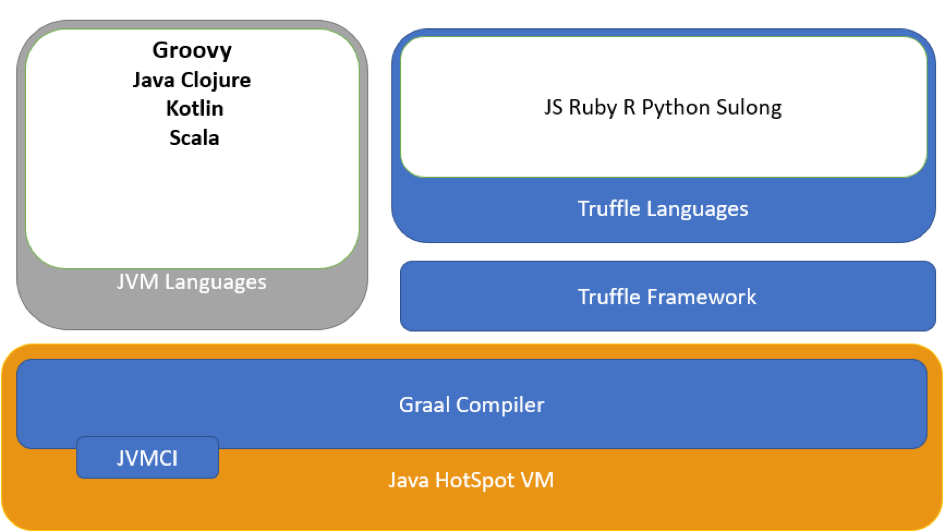
\includegraphics[width=0.7\textwidth]{images/graalvmArchitecture}
        \caption{GraalVM\tiny{(source:beyondjava.net/graalvm-plugin-replacement-to-jvm)}}
        \label{fig:graalvmArchitecture}
    \end{figure}
\end{frame}

\begin{frame}{Truffle in Nutshell}
        Language Implementation Framework:
        \begin{itemize}
            \vspace{3mm}
            \item It developers to create self-optimizing AST interpreters in Java.
        \end{itemize}
        \vspace{3mm}
        Partial Evaluator:
        \begin{itemize}
            \vspace{3mm}
            \item Uses profiling information to apply speculative optimization.
            \vspace{3mm}
            \item The interpreter get partially evaluated w.r.t the \textbf{hot} parts of the AST.
        \end{itemize}
\end{frame}

%partial eval
\begin{frame}{Partial Evaluation of User Program}
    \begin{figure}[h]
        \centering
        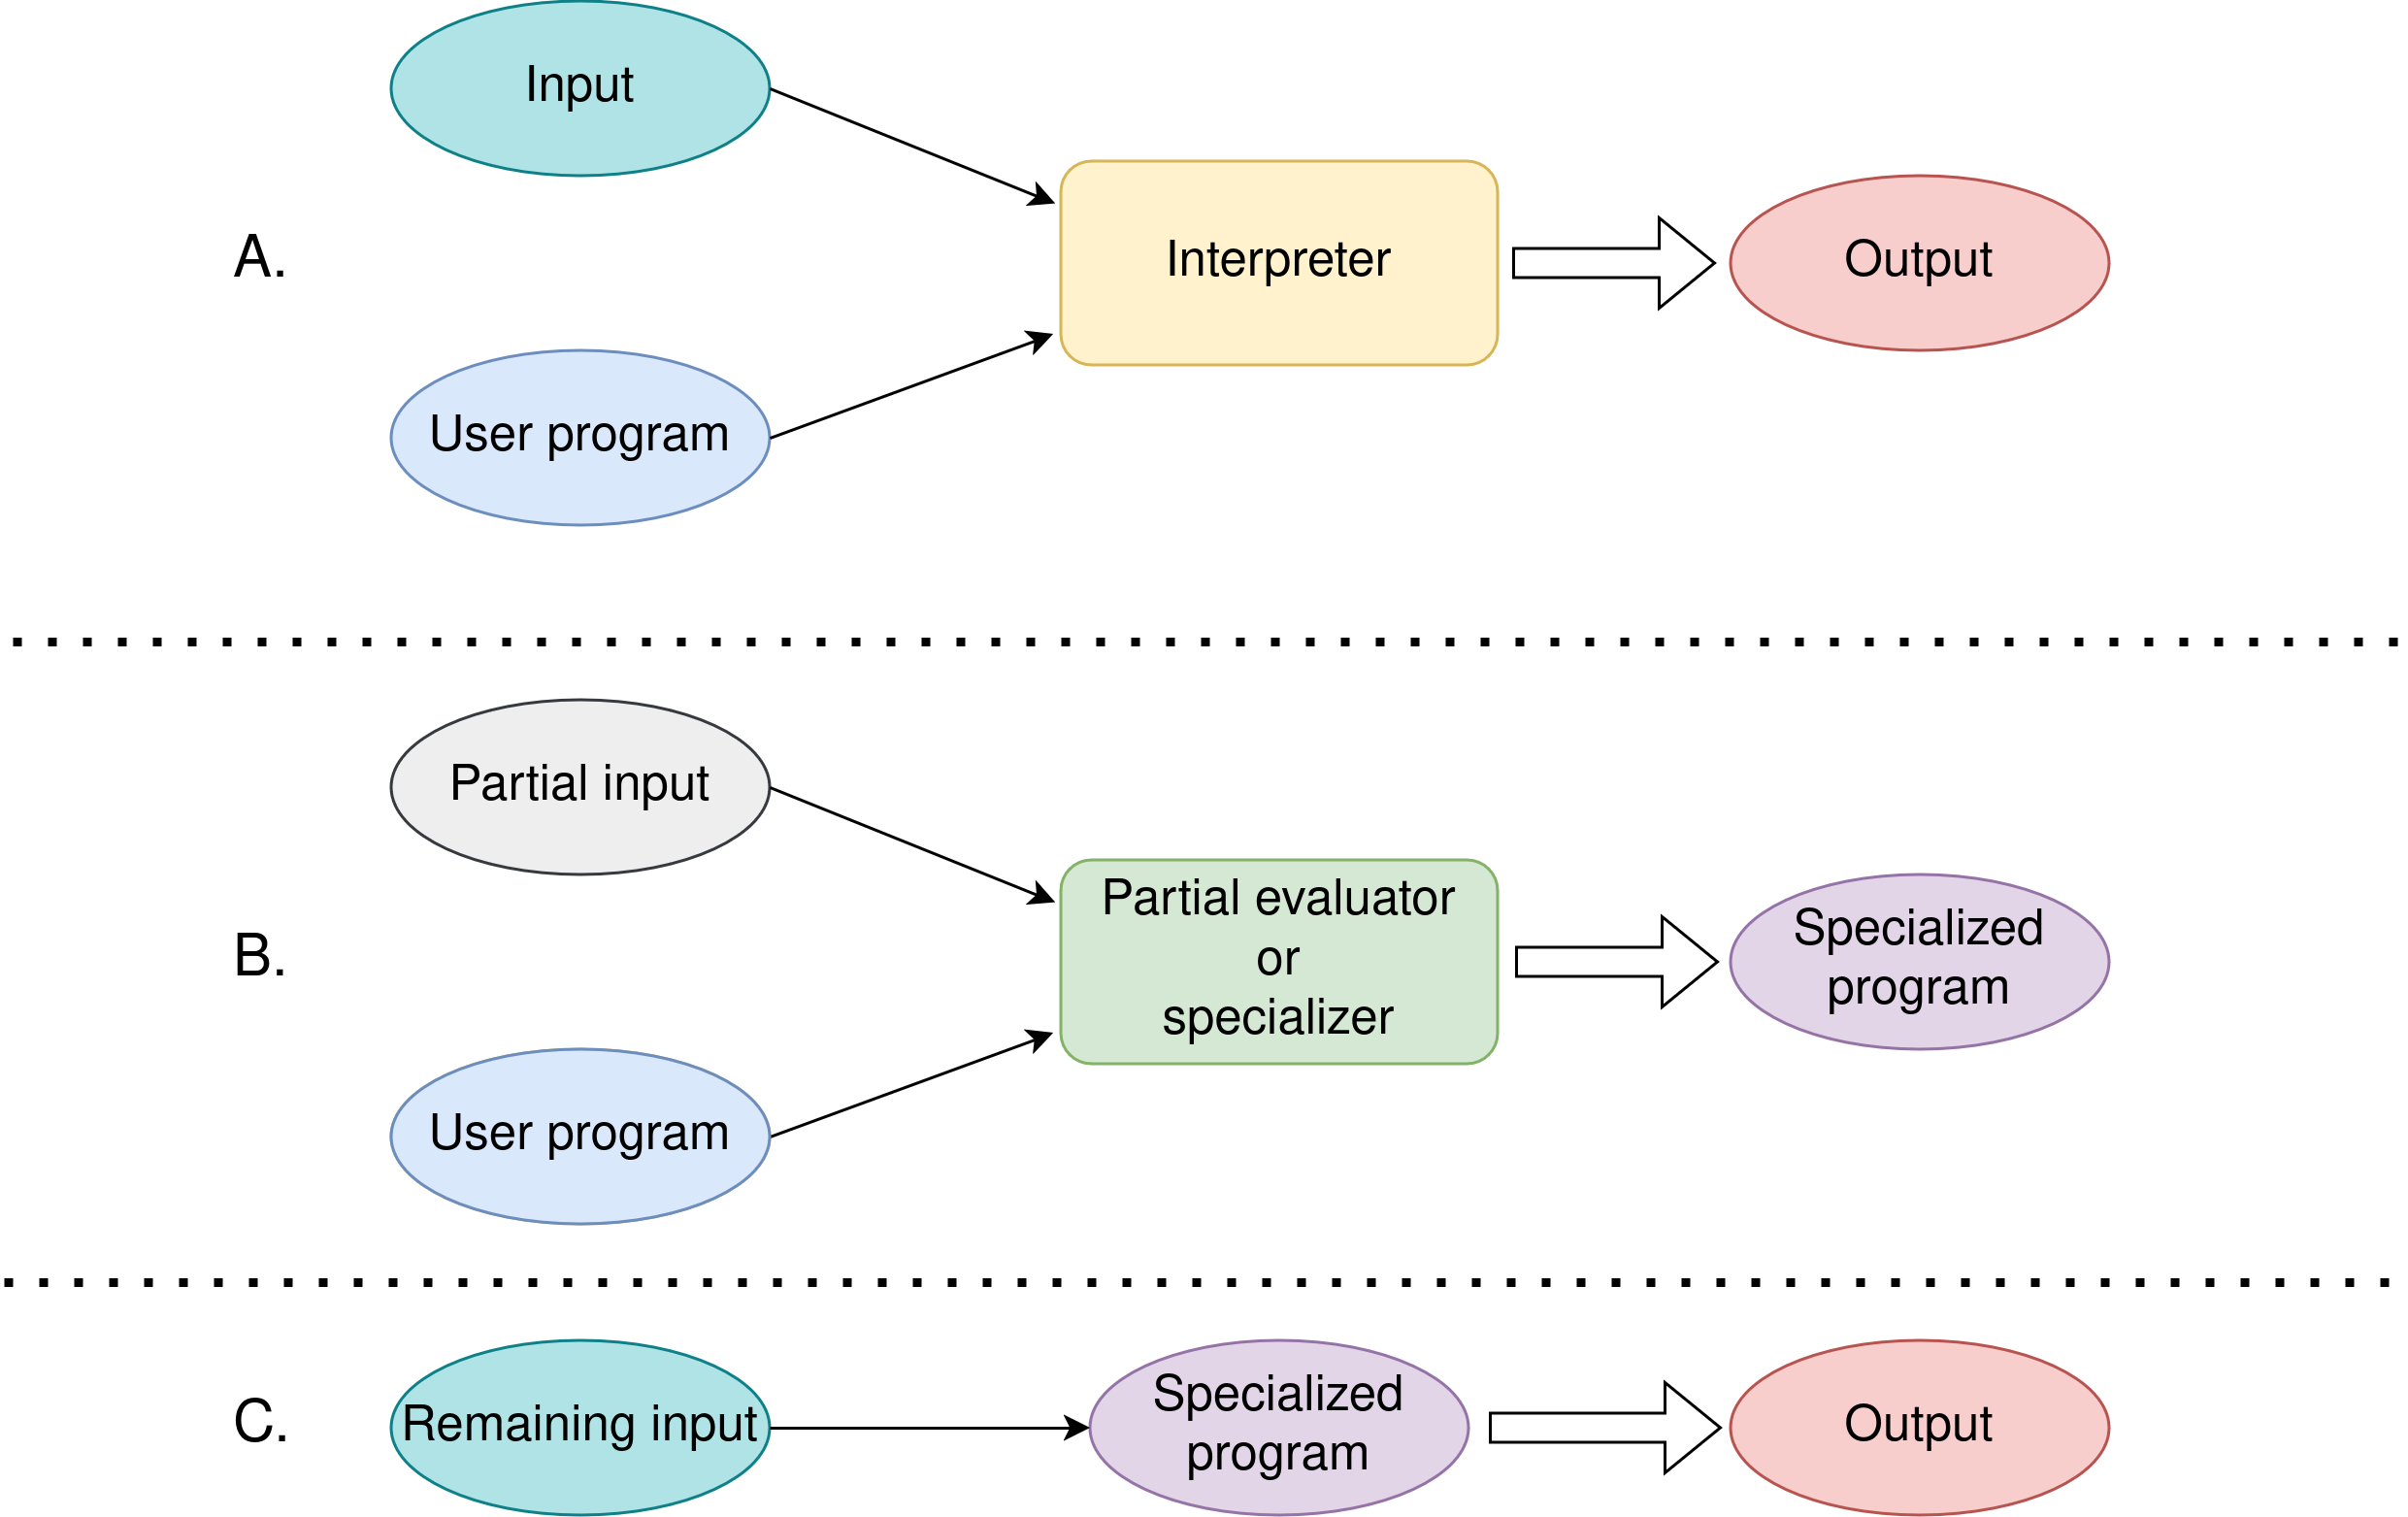
\includegraphics[width=0.6\textwidth]{images/partial-eval-of-program}
        \caption{\textbf{A)} Normal working of interpreter \textbf{B)} Specialization of program \textbf{C)} Faster code}
    \end{figure}
\end{frame}
\begin{frame}{Partial Evaluation of AST Interpreter}
    \begin{figure}[h]
        \centering
        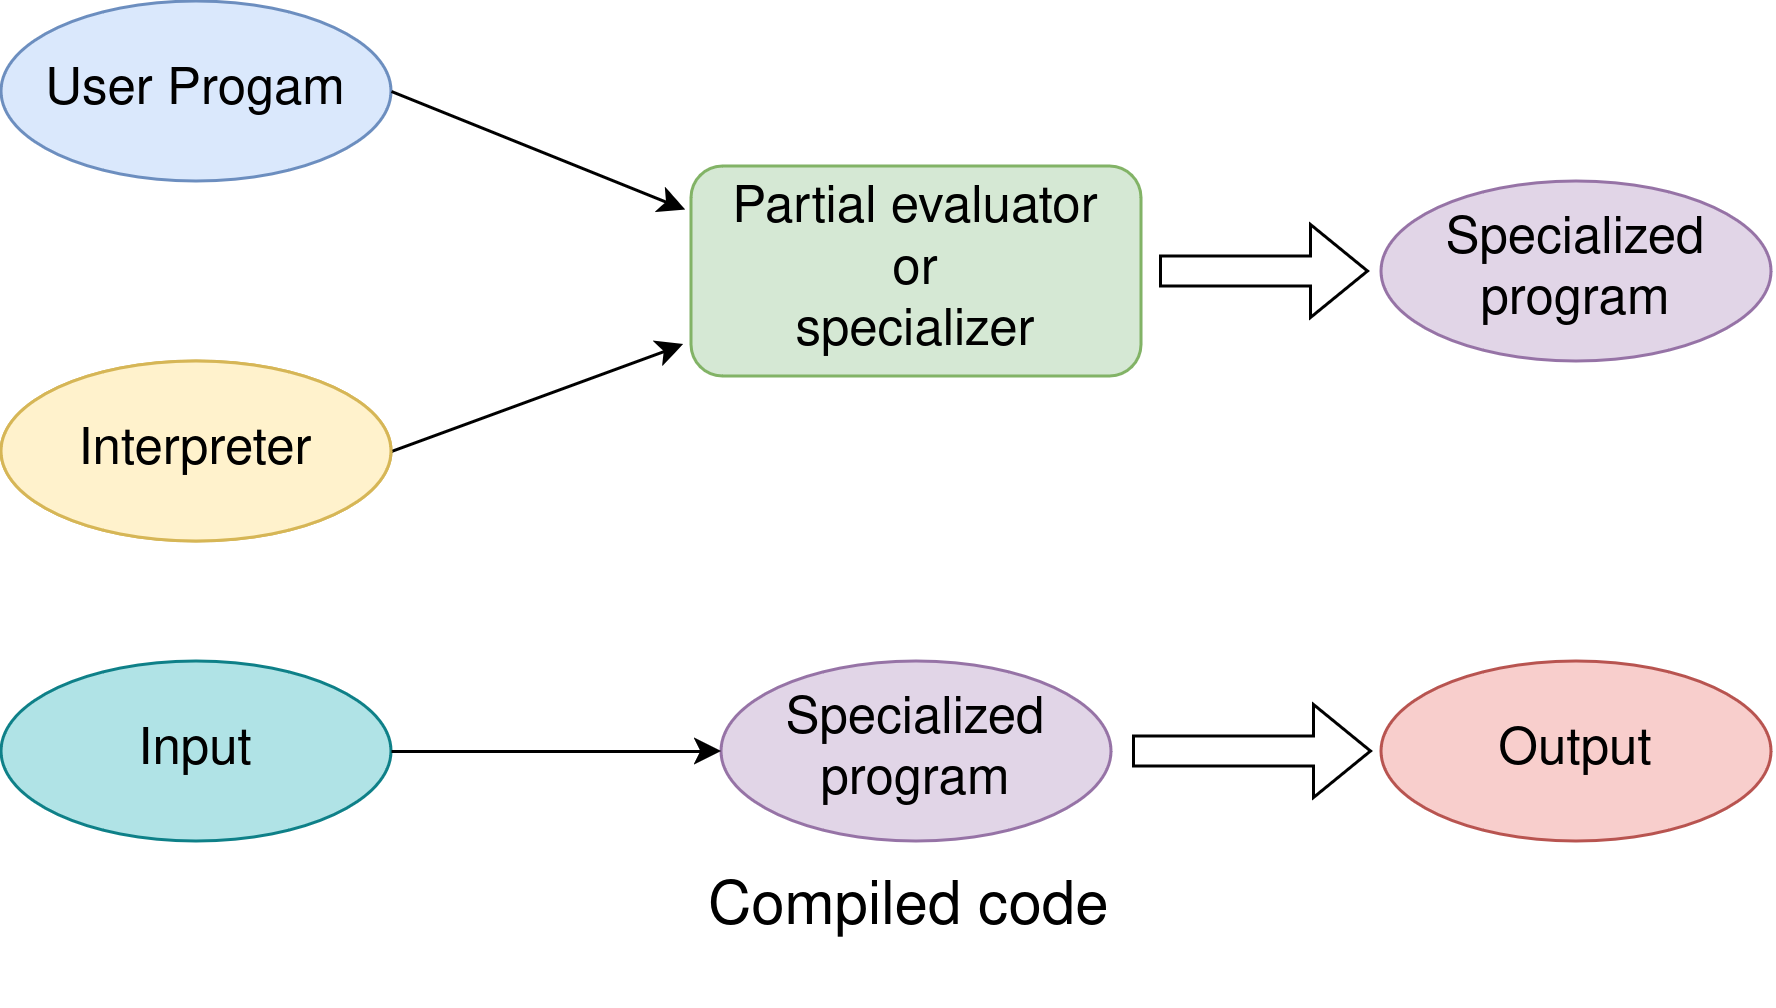
\includegraphics[width=0.6\textwidth]{images/partial-eval-of-interpreter.png}
        \caption{Partially evaluation the AST interpreter with respect to user program}
    \end{figure}
\end{frame}


    \section{Java Native Interface, a Polyglot System?}
    % jni_static_analysis.tex
\begin{frame}
    \centering
    \textbf\ttfamily{\huge{Java Native Interface}}
\end{frame}

\begin{frame}{Java Native Interface}
    \begin{itemize}
        \vspace{3mm}
        \item The Java Native Interface (JNI) acts as a bridge between Java and native languages.
        \vspace{3mm}
        \item Enables Java programs to leverage the advantages of native code.
        \vspace{3mm}
        \item Similar to polyglot systems but does not have a shared runtime.
    \end{itemize}
\end{frame}


\begin{frame}[fragile]{Example of JNI in Java}
    \begin{center}
        \begin{minipage}{0.8\textwidth} % Adjust width as needed
            \begin{lstlisting}[language=java,
                frame=single,
                numbers=left,
                basicstyle=\tiny\ttfamily,
                caption={Vector arithmetic  },
                captionpos=b,
                backgroundcolor=\color{lightgray},   % Background color
                numberstyle=\color{pink},            % Line number color
                keywordstyle=\color{keywordcolor}\bfseries, % Keywords color
                commentstyle=\color{commentcolor},   % Comment color
                stringstyle=\color{stringcolor}      % String color
            ,label={lst:lstlisting}]
public class Main {
    static { // Load the native library
        System.loadLibrary("Polynative");
    }
    // Declare the native method for addition
    public native Vectors add(Vectors a,Vectors b);

    public static void main(String[] args) {
        Vectors p1 = new Vectors(31, 2);    //O9
        Vectors p2 = new Vectors(4, 54);    //O10

        Main caller=new Main();             //O12
        Vectors result1 = caller.add(p1,p2);  // Add p1 and p2
        result1.display();

        for (int i = 0; i < 10000; i++) {
            Vectors temp = new Vectors(i*i, 3*i); //O17
            Vectors sum = caller.add(p1,temp);
            sum.display();
        }
    }
}
            \end{lstlisting}
        \end{minipage}
    \end{center}
%    This example shows a Java HashMap being passed to a Python function, which retrieves and prints values.
\end{frame}

\begin{frame}{Escape Analysis in Java}
    Object is said to be escaping from its allocating method if and only if:
    \begin{itemize}
        \vspace{3mm}
        \item Object is assigned to a static(global) var.
        \vspace{3mm}
        \item It is accessible from another thread.
        \vspace{3mm}
        \item It is reachable via some chain of field dereferences.
        \vspace{3mm}
        \item Passed to a method as parameter which cannot be analyzed.
    \end{itemize}
\end{frame}

\begin{frame}{Escape Analysis in JNI Programs}
    We modified an existing$_2$ inter-procedural escape analysis to collect the following information:
    \begin{itemize}
        \vspace{3mm}
        \item Recording different types of calls(Static, Virtual, Special and Native).
        \vspace{3mm}
        \item Identifying objects escaped via native calls.
    \end{itemize}
     % Smaller font size for the source
    \vspace{3cm}
    \tiny
    \textit{2: \url{https://github.com/meetesh06/}}
\end{frame}

\begin{frame}{Findings using SOOT Analysis Framework}
    \begin{table}[H]
        \label{tab:jni_analysis_results}
        \begin{tabular}{|l|c|c|c|c|c|c|}
            \hline
            \textbf{Parameters} & \textbf{avrora} & \textbf{h2} & \textbf{batik}  & \textbf{helloWorld} & \textbf{myJNI} \\
            \hline
            Classes loaded          & 674  & 753  & 927  & 809  & 811  \\
            Interface calls          & 1499  & 2159  & 1360  & 6586  & 6857  \\
            Special calls           & 1745  & 2062  & 2840   & 2314  & 2329  \\
            JNI calls               & 42   & 53   & 54    & 65   & 65   \\
            Virtual calls           & 11206 & 13027 & 14293  & 13358 & 14826 \\
            Static calls            & 1124 & 1288  & 1715  & 1283  & 1286  \\
            Total objects          & 934  & 1122  & 1068  & 1210  & 1223 \\
            Escaped objects         & 531  & 459  & 768    & 569  & 574  \\
            Escaped via JNI         & 180   & 82   & 302     & 151   & 151   \\
            \% Escaped via JNI     & 33\%  & 17\%  & 39\%   & 26\%  & 26\%   \\
            Methods analyzed        & 2987 & 3539 & 4310 & 4033 & 4051 \\
            \hline
        \end{tabular}
        \caption{Results for some popular benchmark from $Dacapo$ \& custom programs}
    \end{table}

\end{frame}

\begin{frame}{Summary}
       \begin{itemize}
        \vspace{3mm}
        \item Experiment revealed that JNI calls are relatively rare.
        \vspace{3mm}
        \item The number of escaped objects through JNI calls were significant($~28\%$).
        \vspace{3mm}
        \item A $Hello world!$ program implicitly invokes JNI methods via java libraries.
        \vspace{3mm}
        \item These calls make results imprecise, since analysis is limited by language boundary.
        \vspace{3mm}
        \item If we could incorporate native methods analysis, optimization techniques could be improved.
    \end{itemize}
\end{frame}


    \section{A Common Interface for Polyglot Systems}
    % polyglot_optimization.tex
\begin{frame}
    \centering
    \textbf\ttfamily{\huge{A Common Interface}}
\end{frame}

\begin{frame}{Analyses and Challenges}
    \begin{figure}[h]
        \centering
        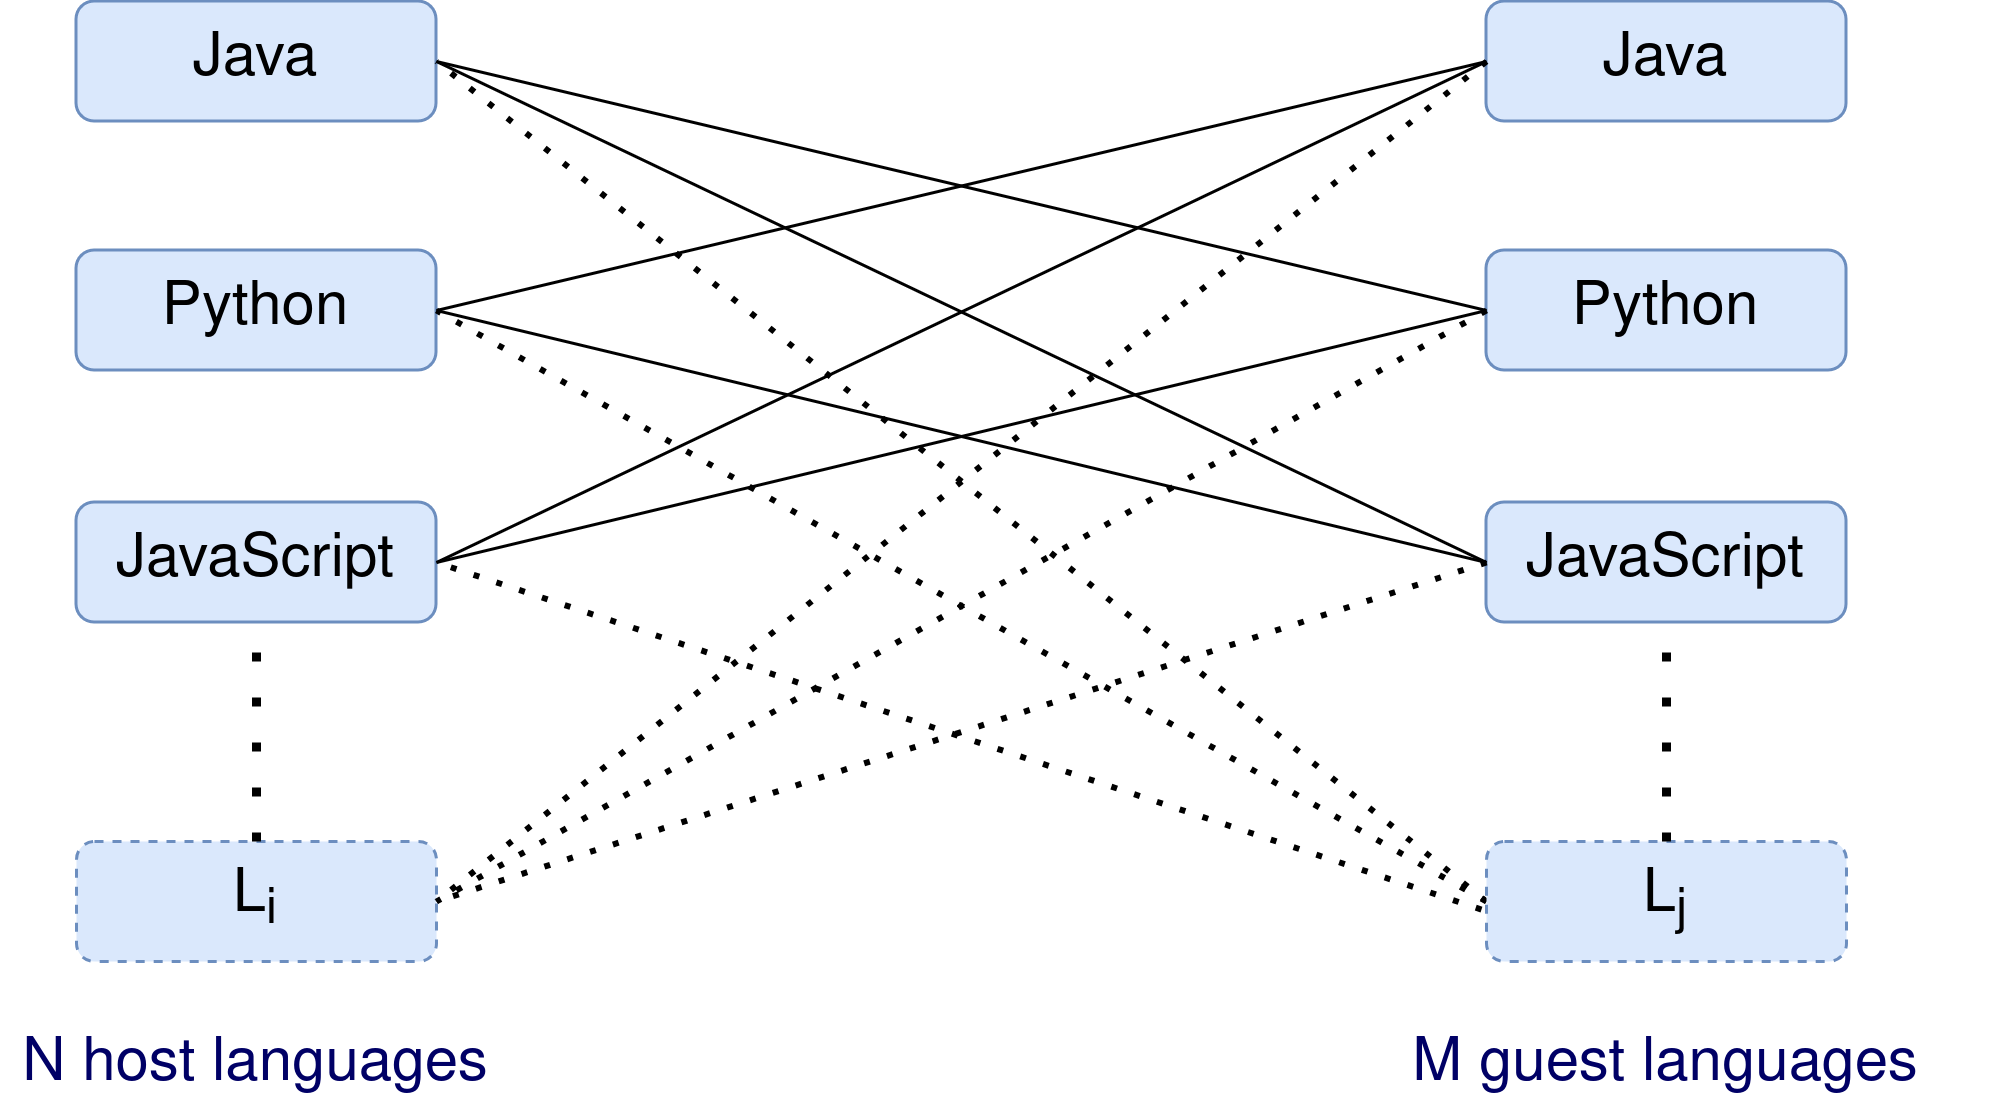
\includegraphics[width=0.6\textwidth]{images/nxm analyses}
        \caption{$NxM$ polyglot systems}
        \label{fig:figure}
    \end{figure}
    \begin{itemize}
        \item To analyze polyglot programs, one need to run interlanguage analyses.
    \end{itemize}
\end{frame}

\begin{frame}{Possible Solutions}
    \begin{itemize}
        \item Several approaches were considered for polyglot program analysis:
        \begin{enumerate}
            \vspace{3mm}
            \item Translate the guest languages to host languages.
            \vspace{3mm}
            \item Develop a new IR that can express all languages.
            \vspace{3mm}
            \item Use an existing interface that is compatible with both host and guest languages.
        \end{enumerate}
    \end{itemize}
\end{frame}


\begin{frame}[fragile]{Previous Example: Java calling Python Script}
    \begin{minipage}[b]{0.45\linewidth}
        \centering
        \begin{lstlisting}[
            frame=single,
            language=python,
            numbers=left,
            basicstyle=\tiny\ttfamily,
            caption={\normalsize{Adding complex no. in loop}},
            captionpos=b,
            backgroundcolor=\color{lightgray},   % Background color
            numberstyle=\color{pink},            % Line number color
            keywordstyle=\color{keywordcolor}\bfseries, % Keywords color
            commentstyle=\color{commentcolor},   % Comment color
            stringstyle=\color{stringcolor}      % String color
        ,label={lst:lstlisting2}]
class ComplexNumber:
def __init__(self, r, i):
    self.r = r
    self.i = i
def __add__(self, other):
    cTmp= ComplexNumber(self.r, other.i)
    return ComplexNumber(self.r+other.r+cTmp.r,
                         self.i+other.i+cTmp.i)
def __str__(self):
    return f"({self.r} + {self.i}i)"

def addComplex(i:int, n:int):
    c1 = ComplexNumber(545,n)  #python object
    c2 = ComplexNumber(9878,i) #python object
    return c1 + c2

def addComplexLoop(n: int):
    sum=0
    for i in range(10000):
        sum= sum+ addComplex(i,n).r
    return sum
        \end{lstlisting}
    \end{minipage}
    \hspace{6mm}
    \begin{minipage}[b]{0.48\linewidth}
        \centering
        \begin{lstlisting}[
            frame=single,
            language=java,
            numbers=left,
            basicstyle=\tiny\ttfamily,
            caption={Python script called from java},
            captionpos=b,
            backgroundcolor=\color{lightgray},   % Background color
            numberstyle=\color{pink},            % Line number color
            keywordstyle=\color{keywordcolor}\bfseries, % Keywords color
            commentstyle=\color{commentcolor},   % Comment color
            stringstyle=\color{stringcolor}      % String color
        ,label={lst:lstlisting2.1}]
void test() {
    String pyFile=
       "./src/main/polyglot/testCase.py";
    //create a context
    try (Context ctx = Context.create()) {
       File f= new File(pyFile);
       //load the file
       Source src= Source.
                  newBuilder("python",f).build();
       //load the py script in ctx
       ctx.eval(src);
       //getting python function
       Value pyLoop = ctx.getBindings("python")
               .getMember("addComplexLoop");
       //calling python fun
       Value result= pyLoop.execute(1000);
       System.out.println(result.asLong());
    } catch (Exception e) {
       e.printStackTrace();
    }
}
        \end{lstlisting}
    \end{minipage}
\end{frame}

\begin{frame}{Research Work}
    Our research focused on finding an existing common interface:
    \begin{itemize}
        \vspace{2mm}
        \item Experimented with Java-Python polyglot system.
        \vspace{2mm}
        \item Constructed various test programs.
        \vspace{2mm}
        \item Visually analyzed compilation graphs at different tiers of Graal and Truffle.
    \end{itemize}
\end{frame}

\begin{frame}{Tools Used}
    We used the following tools to aid us:
    \begin{itemize}
        \item \textbf{Dgraal.Dump} graal compiler flag to dump IRs from different compiler tiers
        \vspace{2mm}
        \item \textbf{Ideal Graph Visualizer(IGV)} was used to visualize the compilation dumps.
        \vspace{2mm}
        \item \textbf{Seaform} was further used to reorganise information from the dumps and remove unwanted information.
    \end{itemize}
\end{frame}
\begin{frame}{Guest Language Object Allocation}
    \begin{figure}[h]
        \centering
        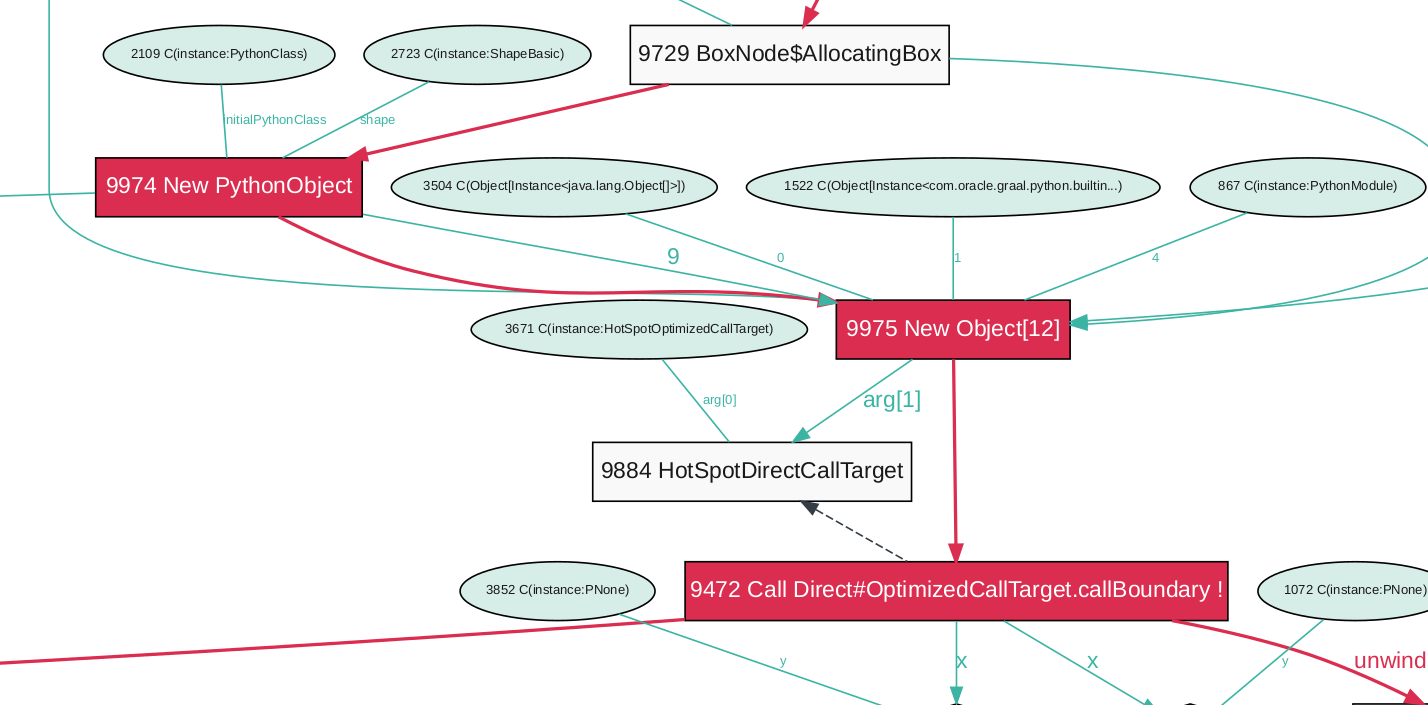
\includegraphics[width=0.8\textwidth]{images/igv_dump}
        \caption{A Python object in the output of PE}
    \end{figure}
\end{frame}
\begin{frame}{Findings}
    \begin{figure}[h]
        \centering
        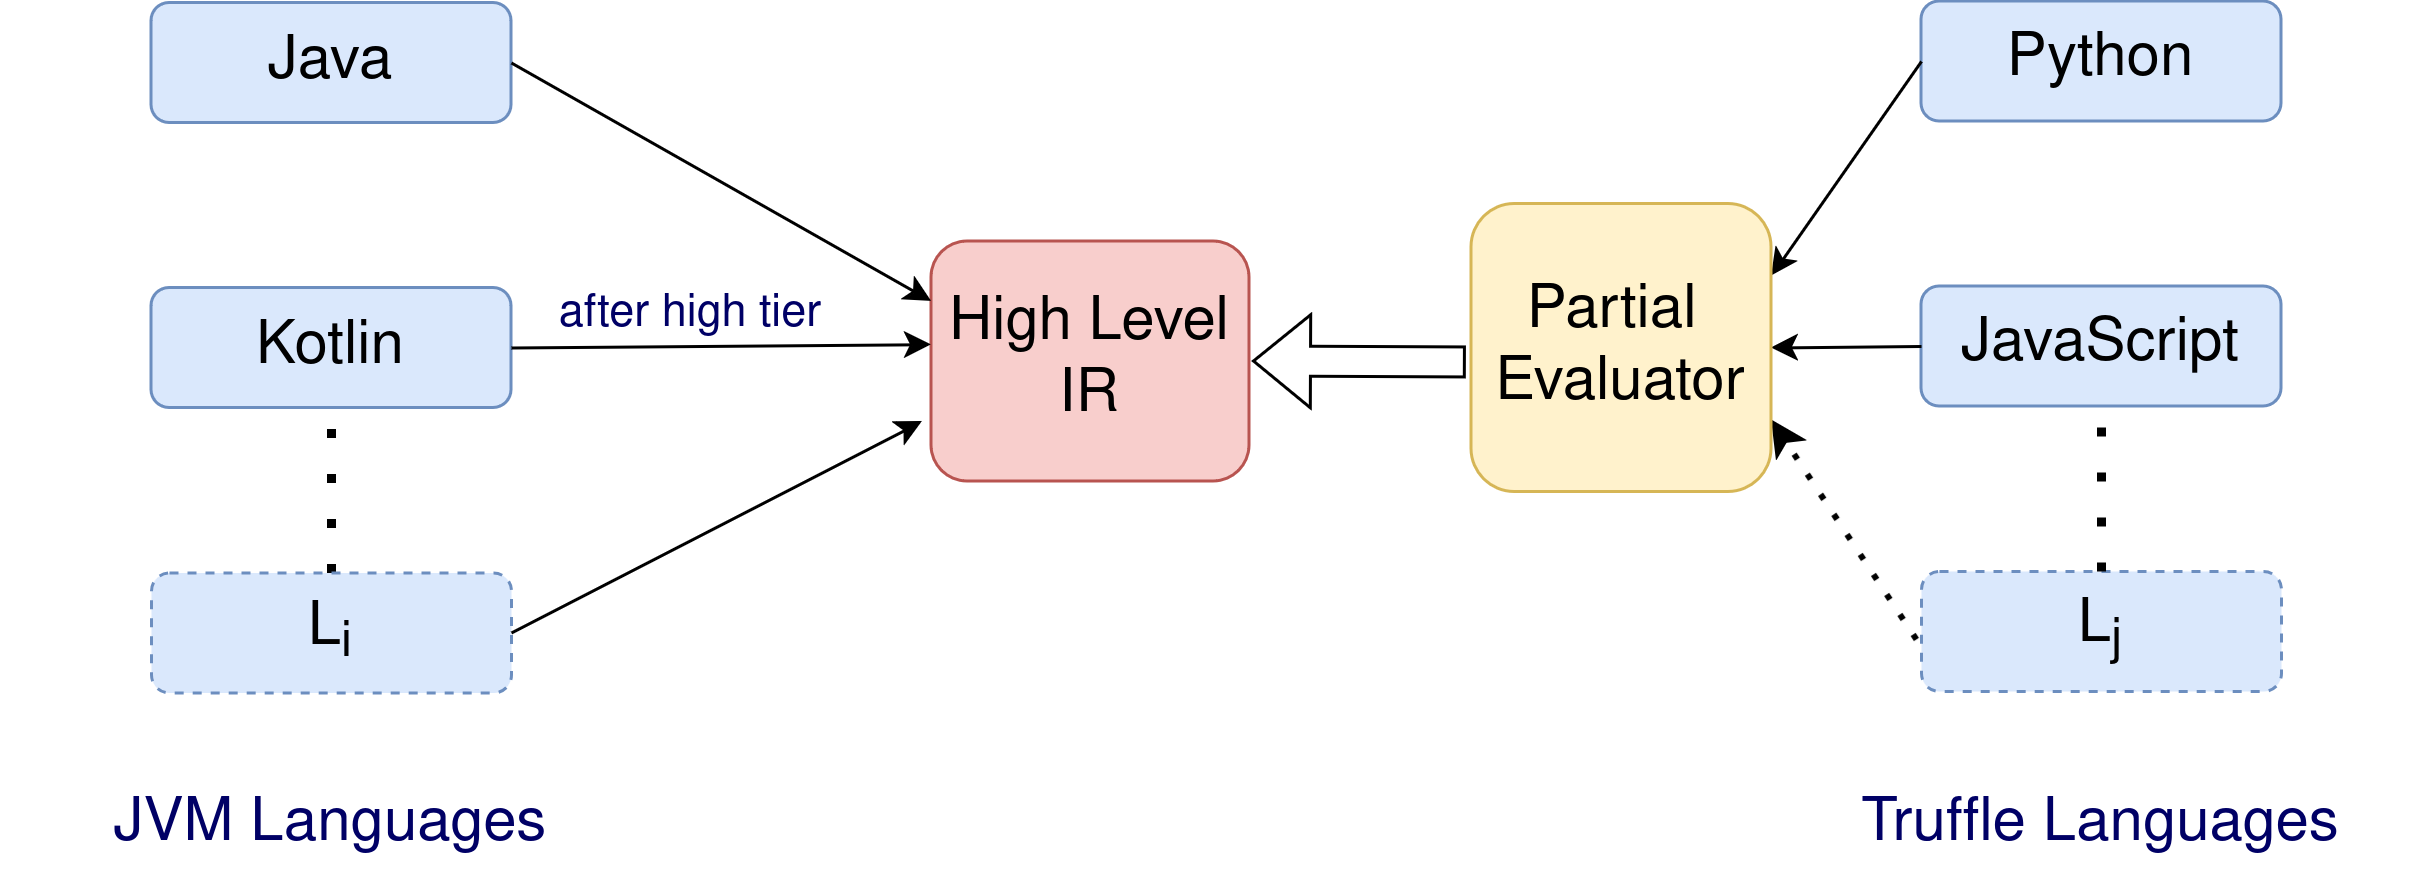
\includegraphics[width=0.6\textwidth]{images/common_interface}
        \caption{$NxM$ polyglot systems with a common interface}\label{fig:figure2}
    \end{figure}

    \begin{itemize}
        \item Truffle PE actually produces High-Level Intermediate Representation (HIR).
    \end{itemize}
\end{frame}
\begin{frame}{Proposed Solution}
    \begin{itemize}
        \item We can utilize this HIR to develop an analysis framework which will facilitate inter-procedural analyses across languages.
        \vspace{2mm}
        \item In the PYE research paper author implemented a similar framework in to make analysis more precise in OpenJDK's JIT.
        \vspace{2mm}
    \end{itemize}
\end{frame}


    \section{Conclusion and Future Work}
    % conclusion_future_work.tex
\begin{frame}
    \centering
    \textbf\ttfamily{\huge{Conclusion}}
\end{frame}

\begin{frame}{Conclusion}
    \begin{itemize}
        \item Language boundaries limit the analyses, making polyglot program optimization challenging.
        \vspace{2mm}
        \item Our research found HIR the most suitable for common interface.
        \vspace{2mm}
        \item We propose to use this HIR to develop an analysis framework for polyglot program optimization.
    \end{itemize}
\end{frame}

\begin{frame}{Future Work}
    \begin{itemize}
        \item This inter-language framework aims to facilitate optimization techniques across language boundaries.
        \vspace{2mm}
        \item Developing a more comprehensive framework that integrates with existing GraalVM system.
        \vspace{2mm}
        \item Evaluating the effectiveness of the proposed framework with real-world applications.
    \end{itemize}
\end{frame}


    \section{References}
    
\begin{frame}{References}
    \begin{itemize}
        \item Thomas Würthinger, Christian Wimmer, Christian Humer, Andreas Wöß, Lukas Stadler, Chris Seaton, Gilles Duboscq, Doug Simon, and Matthias Grimmer. 2017. Practical partial evaluation for high-performance dynamic language runtimes. SIGPLAN Not. 52, 6 (June 2017), 662–676. https://doi.org/10.1145/3140587.3062381
        \vspace{2mm}
        \item Manas Thakur and V. Krishna Nandivada. 2019. PYE: A Framework for Precise-Yet-Efficient Just-In-Time Analyses for Java Programs. ACM Trans. Program. Lang. Syst. 41, 3, Article 16 (September 2019), 37 pages. https://doi.org/10.1145/3337794
        \vspace{2mm}
        \item Jyoti Prakash, Abhishek Tiwari, Christian Hammer. Unifying Pointer Analyses for Polyglot Inter-operations through Summary Specialization. https://arxiv.org/abs/2305.03916
        % Add references here
    \end{itemize}
\end{frame}


    \section{Q\&A}
    % 7_thank_you.tex

\begin{frame}
    \centering
    {\Huge Thank You!}
\end{frame}


    \section{}
    \begin{frame}[fragile]{Native method structure: Template}
    \begin{center}
        \begin{minipage}{0.8\textwidth} % Adjust width as needed
            \begin{lstlisting}[
                language=c,
                numbers=left,
                basicstyle=\tiny\ttfamily,
                caption={Auto generated c++ template by Java},
                captionpos=b,
                backgroundcolor=\color{lightgray},   % Background color
                numberstyle=\color{pink},            % Line number color
                keywordstyle=\color{keywordcolor}\bfseries, % Keywords color
                commentstyle=\color{commentcolor},   % Comment color
                stringstyle=\color{stringcolor}      % String color
            ]
/* DO NOT EDIT THIS FILE - it is machine generated */
#include <jni.h>
/* Header for class Main */

#ifndef _Included_Main
#define _Included_Main
#ifdef __cplusplus
extern "C" {
#endif
/*
 * Class:     Main
 * Method:    add
 * Signature: (LVectors;LVectors;)LVectors;
 */
JNIEXPORT jobject JNICALL Java_Main_add
  (JNIEnv *, jobject, jobject, jobject);

#ifdef __cplusplus
}
#endif
#endif
            \end{lstlisting}
        \end{minipage}
    \end{center}
\end{frame}

\begin{frame}[fragile]{JNI: Native method structure}
    \begin{center}
        \begin{minipage}{0.8\textwidth} % Adjust width as needed
            \begin{lstlisting}[
                language=c,
                numbers=left,
                basicstyle=\tiny\ttfamily,
                caption={Native method implemenation in c++},
                captionpos=b,
                backgroundcolor=\color{lightgray},   % Background color
                numberstyle=\color{pink},            % Line number color
                keywordstyle=\color{keywordcolor}\bfseries, % Keywords color
                commentstyle=\color{commentcolor},   % Comment color
                stringstyle=\color{stringcolor}      % String color
            ]
JNIEXPORT jobject JNICALL Java_Main_add
  (JNIEnv *env, jobject caller, jobject v1, jobject v2){

    jclass numberClass=env->GetObjectClass( v1); //to get the class

    jfieldID fieldID_x=env->GetFieldID(numberClass,"x","D");
    jfieldID fieldID_y=env->GetFieldID(numberClass,"y","D");

    //get the field by its field id from the object p
    jdouble x1=env->GetDoubleField(v1,fieldID_x);
    jdouble x2=env->GetDoubleField(v2,fieldID_x);

    jdouble temp_r= x1+x2;

    //find the method ID of constructor of NumberClass
    jmethodID numberClass_init_id=env->GetMethodID(numberClass,"<init>","(DD)V");

    //create an object of NumberClass type
    jobject temp_obj=env->NewObject(numberClass,numberClass_init_id,temp_r,temp_i);

    return temp_obj;
  }
            \end{lstlisting}
        \end{minipage}
    \end{center}
\end{frame}



\end{document}
